% !TEX TS-program = XeLaTeX
% !TEX encoding = UTF-8 Unicode

\chapter{实验设计与结果分析}
\label{chap:experiment}
\defaultfont

\section{实验目标}
实验部分围绕基于 WiFi CSI 的脊柱姿态检测方法展开，验证接收天线相位比、文件级统计特征和 ExtraTrees 分类器在三类姿态识别任务中的有效性。实验目标包括：检验 CSI 相位比特征是否能够反映不同脊柱姿态差异；比较 TCN、SVM、Random Forest 和 ExtraTrees 等模型的分类效果；分析最终模型在测试集上的准确率、精确率、召回率、F1 值和混淆矩阵表现。

\section{研究问题}
为了使实验过程与研究目标相对应，本文将评价内容归纳为三个研究问题。第一个问题是，在统一的数据划分条件下，基于文件级统计特征的传统分类模型能否获得稳定的三分类结果；第二个问题是，ExtraTrees 与其他候选模型相比是否具有更好的留出测试表现；第三个问题是，不同类别的错误分布是否存在明显差异，以及这些差异能够说明哪些方法局限。

上述问题分别对应方法可行性、模型选择和错误解释三个层面。实验结果只能在给定受试者和相近采集条件下回答这些问题，不能直接证明模型已经具备跨人员、跨环境或临床应用能力。对实验结论的适用范围进行限定，是保证评价结果不被过度解释的重要前提。

\section{数据集与划分方式}
实验数据集共包含 750 个 CSI 原始文件，类别包括 \texttt{kyphosis}、\texttt{normal} 和 \texttt{scoliosis}，分别对应脊柱后凸相关姿态、正常姿态和脊柱侧弯相关姿态。三类样本数量均为 250 个，数据来自 5 位受试者。

图~\ref{fig:dataset_composition} 按受试者与姿态类别展示了原始文件构成。每位受试者在三种姿态下均采集 50 个文件，因而类别与受试者维度均保持平衡，可减少由样本数量差异造成的评价偏差。

\begin{figure}[htbp]
\centering
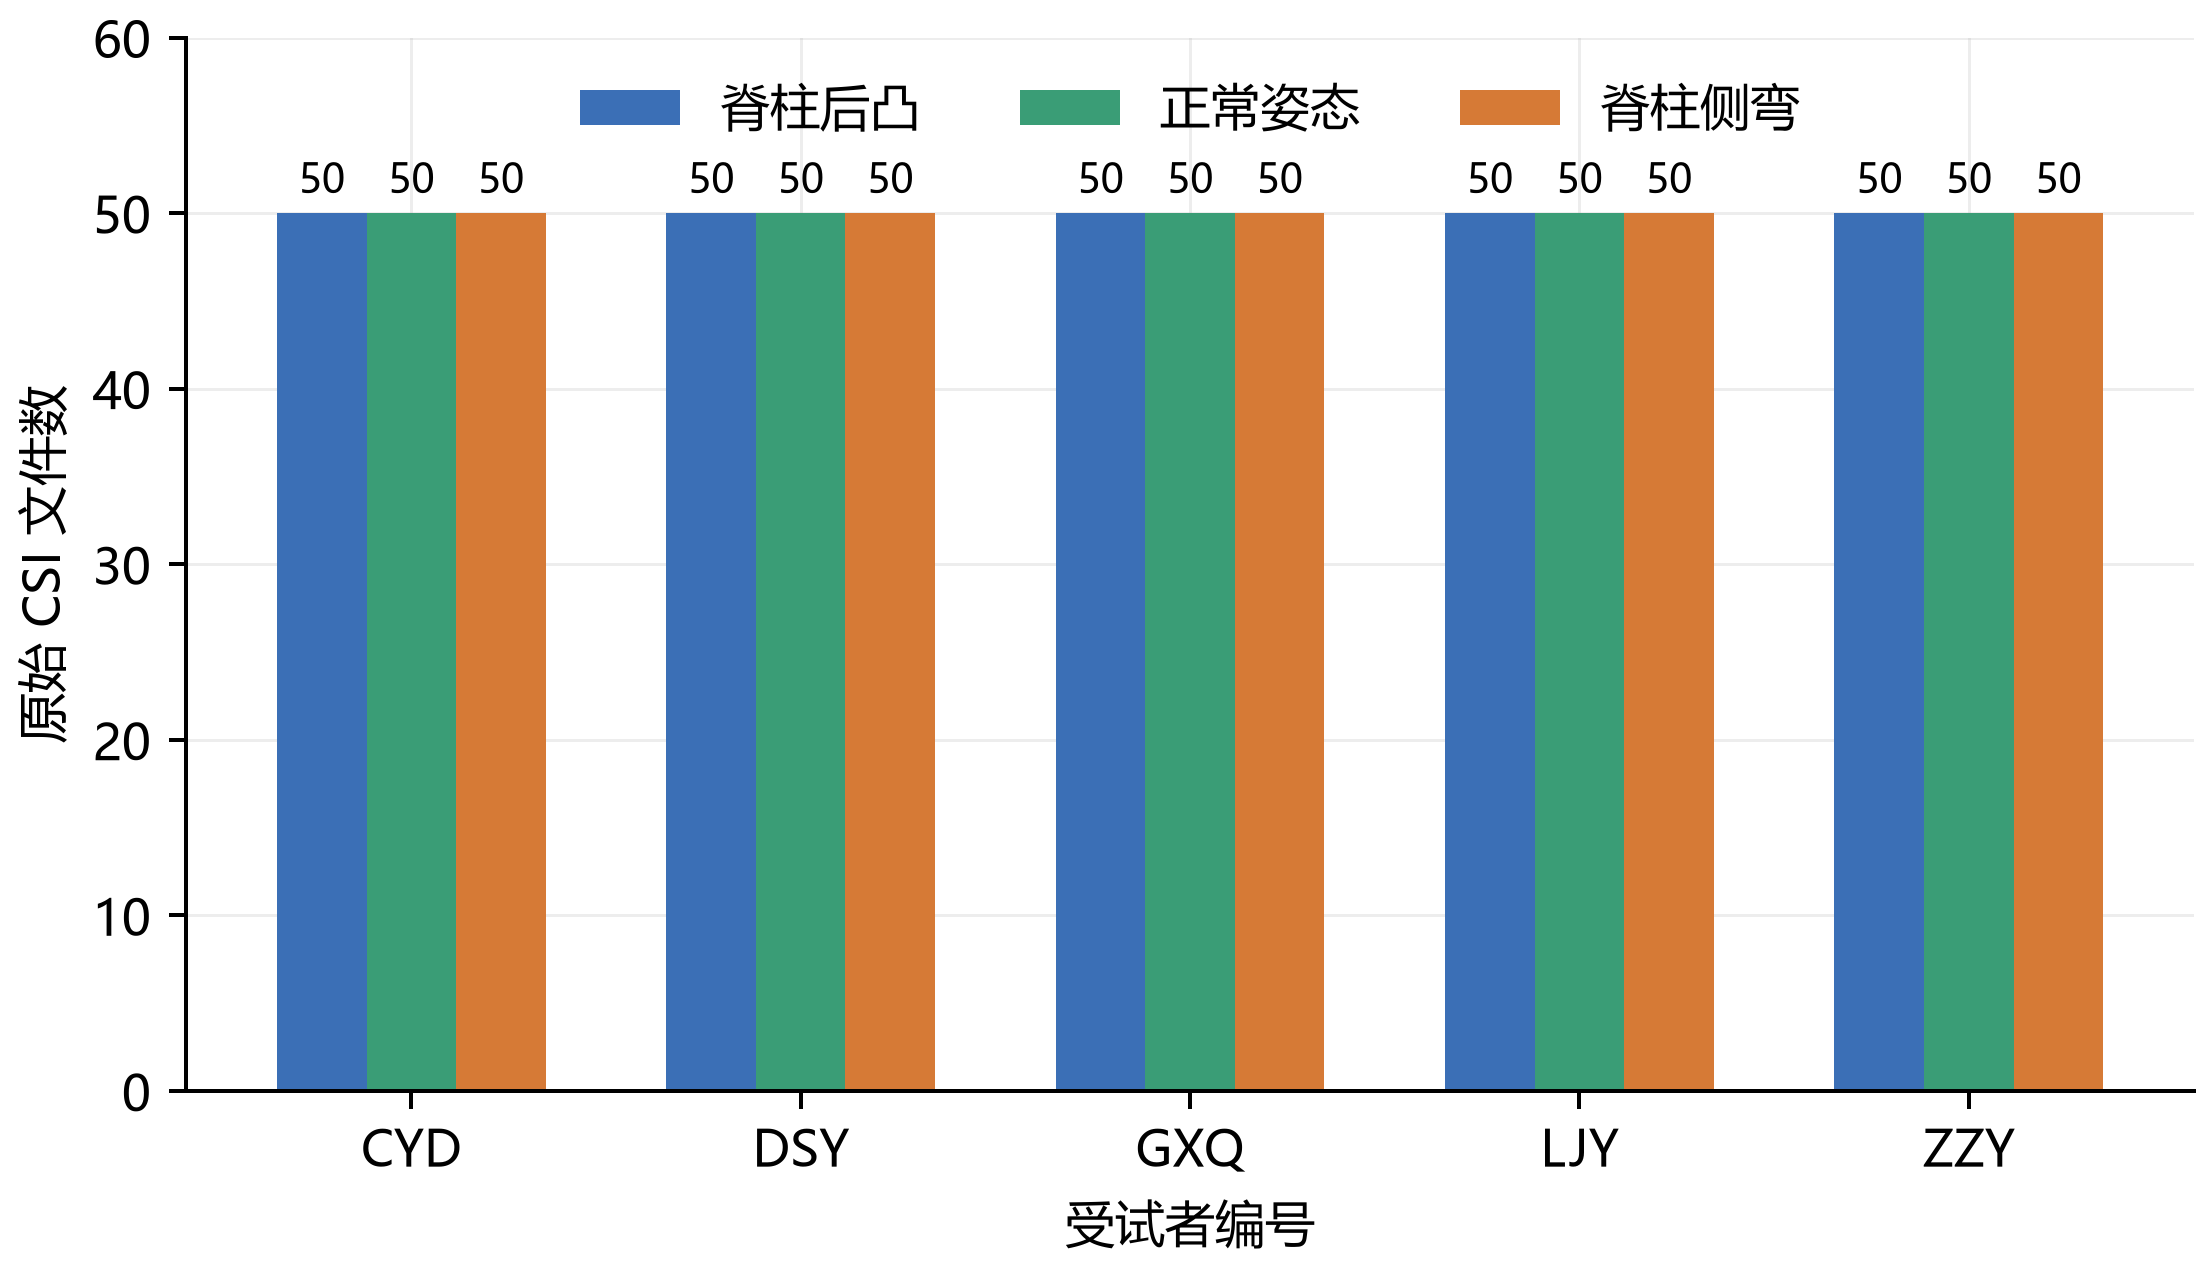
\includegraphics[width=0.88\textwidth]{figures/dataset_composition.png}
\caption{不同受试者与姿态类别的 CSI 文件数量}
\label{fig:dataset_composition}
\end{figure}

数据集采用固定随机种子 42 在原始文件级别进行划分。训练集包含 524 个文件，占 69.9\%；验证集包含 113 个文件，占 15.1\%；测试集包含 113 个文件，占 15.1\%。划分发生在滑动窗口生成之前，因此同一原始文件产生的重叠窗口不会同时出现在训练集和测试集中。

\begin{table}[htbp]
\centering
\song\wuhao
\caption{数据集划分情况}
\label{tab:dataset_split}
\begin{tabular}{cccc}
\hline
数据集 & 文件数 & 比例 & 用途 \\
\hline
训练集 & 524 & 69.9\% & 模型参数学习 \\
验证集 & 113 & 15.1\% & 模型选择与配置比较 \\
测试集 & 113 & 15.1\% & 最终性能评估 \\
\hline
\end{tabular}
\end{table}

各子集内部的类别数量如图~\ref{fig:dataset_split} 所示。训练、验证和测试子集均近似保持三类均衡，其中测试集三类文件数分别为 37、38 和 38。

\begin{figure}[htbp]
\centering
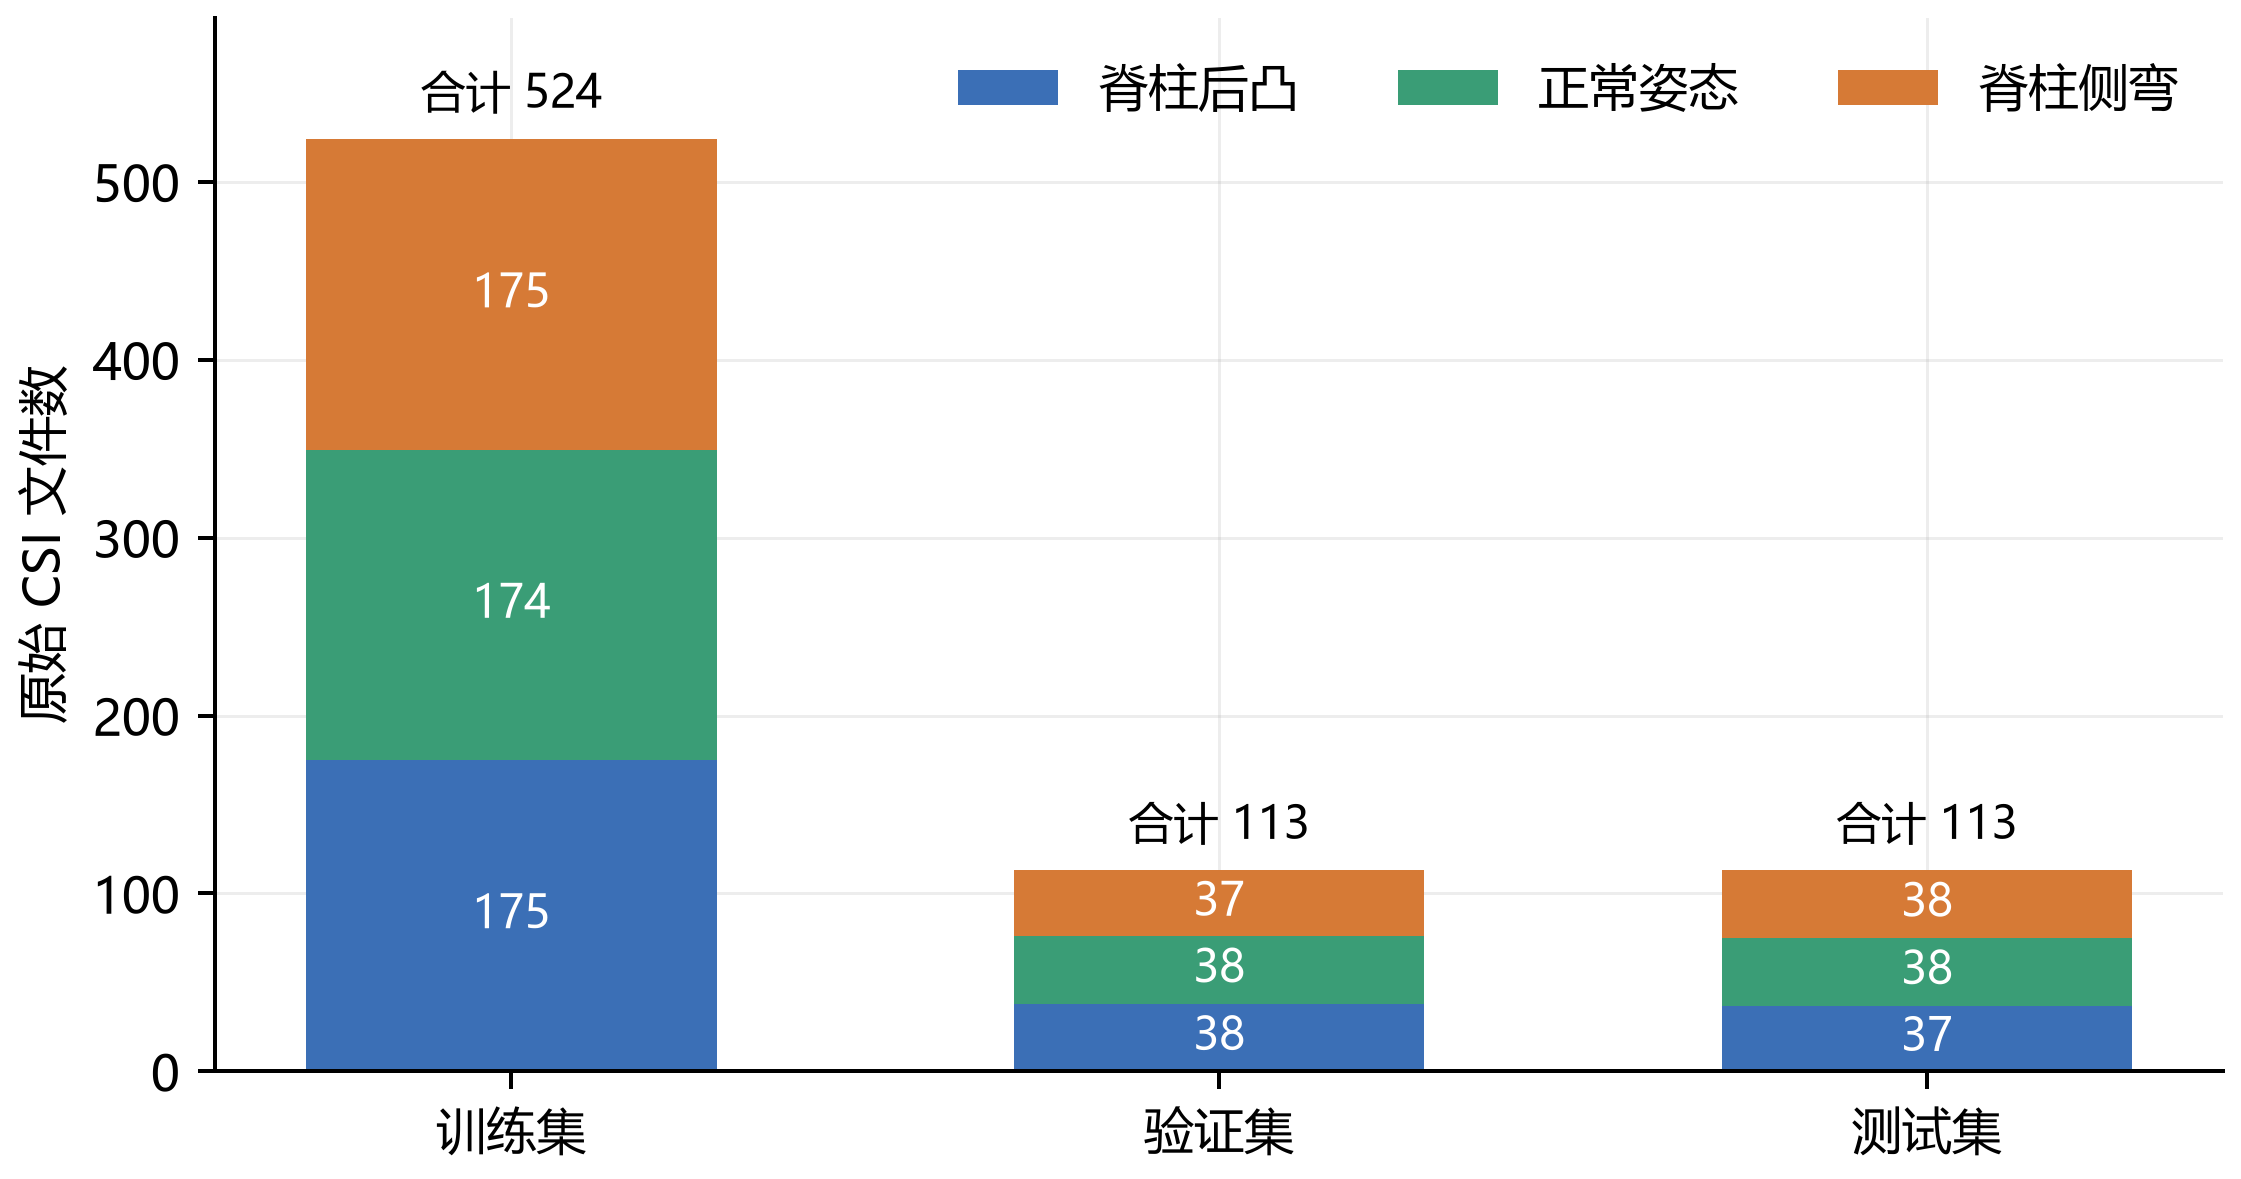
\includegraphics[width=0.82\textwidth]{figures/dataset_split.png}
\caption{训练集、验证集与测试集的类别分布}
\label{fig:dataset_split}
\end{figure}

\section{实验协议与信息隔离}
实验协议按照训练、验证和测试三个阶段组织。训练集用于学习分类模型的参数；验证集用于比较候选模型及其配置；测试集在模型方案确定前保持隔离，仅用于报告最终性能。所有滑动窗口和文件级特征均在原始文件划分完成后生成，避免同一文件产生的重叠窗口进入不同数据子集。

对于 TCN 与传统分类模型的比较，需要注意两类方法的输入单位不同。TCN 使用局部时间窗口，文件级模型使用完整采集文件的统计表示，因此对比结果反映的是“表示方式与分类器组合”的整体差异，而不能仅归因于分类器结构。本文保留该对比用于说明不同建模路线在当前数据条件下的实际表现，同时在结果解释中避免把差异简单表述为某一类模型在所有 CSI 任务中普遍更优。

实验过程中还应保持标签映射、特征维度、随机种子和评价脚本一致。模型配置只能依据训练集与验证集确定，测试集上的分类报告、混淆矩阵和汇总指标由同一组预测结果计算。通过保存数据划分和模型配置，可以在独立运行时重新生成评价结果，并检查训练阶段与检测阶段是否采用一致的数据处理流程。

\section{评价指标}
为了全面评价模型分类效果，实验采用准确率、精确率、召回率和 F1 值作为主要指标。准确率表示预测正确的样本占总样本的比例：
\begin{equation}
Accuracy=\frac{TP+TN}{TP+TN+FP+FN}.
\end{equation}

精确率表示被预测为某一类别的样本中真实属于该类别的比例：
\begin{equation}
Precision=\frac{TP}{TP+FP}.
\end{equation}

召回率表示真实属于某一类别的样本中被正确识别的比例：
\begin{equation}
Recall=\frac{TP}{TP+FN}.
\end{equation}

F1 值综合衡量精确率和召回率：
\begin{equation}
F1=\frac{2\times Precision\times Recall}{Precision+Recall}.
\end{equation}

此外，实验使用混淆矩阵分析不同姿态类别之间的误分情况。混淆矩阵能够直观展示每个真实类别被预测为各类别的数量，有助于观察模型在哪些类别之间更容易混淆。

对于多分类任务，精确率、召回率和 F1 值可以分别按类别计算，再采用宏平均或加权平均形成总体指标。宏平均对每个类别赋予相同权重，适合观察类别均衡条件下的整体表现；加权平均则按照各类别样本数量加权。本文数据集类别数量近似均衡，因此准确率与宏平均指标可以相互补充，但仍需结合逐类结果和混淆矩阵分析，避免单一汇总数值掩盖特定类别的系统性错误。

\section{模型配置选择原则}
候选模型的配置选择遵循“训练集拟合、验证集选择、测试集确认”的原则。对于支持向量机，需要关注核函数、正则化强度和核参数；对于树集成模型，需要关注树数量、候选特征数量、类别权重和叶节点约束；对于时序神经网络，还需要考虑网络深度、感受野、优化过程和早停策略。不同模型的参数含义不同，不宜通过比较参数数量判断其复杂程度。

验证集性能最高并不必然意味着模型具有最好的测试泛化能力。当多个配置的验证结果接近时，应优先考虑结果稳定、结构较简单且计算开销可控的方案。测试集只用于在方案确定后进行一次独立确认，不应根据测试结果继续修改特征或模型，否则测试集会逐渐承担验证集的作用，导致最终性能估计偏乐观。

\section{模型对比实验}
为确定最终分类模型，本文比较了 TCN、RBF SVM、Random Forest 和 ExtraTrees 四种方案。TCN 为早期窗口级深度学习基线，输入为 512 帧 CSI 窗口；SVM、Random Forest 和 ExtraTrees 均使用文件级相位比统计特征。模型对比结果如表 4.2 所示。

\begin{table}[htbp]
\centering
\song\wuhao
\caption{不同模型实验结果对比}
\label{tab:model_compare}
\begin{tabular}{ccccc}
\hline
模型 & 输入单位 & 验证准确率 & 测试准确率 & 测试宏平均 F1 \\
\hline
TCN & 512 帧窗口 & 56.12\% & 50.30\% & 50.16\% \\
RBF SVM & 文件统计特征 & 约 92.04\% & 约 89.38\% & -- \\
Random Forest & 文件统计特征 & 约 96.46\% & 约 90.27\% & -- \\
ExtraTrees & 文件统计特征 & 95.58\% & 92.04\% & 92.08\% \\
\hline
\end{tabular}
\end{table}

图~\ref{fig:model_comparison} 对表~\ref{tab:model_compare} 中的验证和测试准确率作了直观比较。采用文件级统计特征的三种传统模型均明显优于窗口级 TCN；ExtraTrees 的验证结果略低于 Random Forest，但取得最高的测试准确率，显示出更好的留出集泛化表现。

\begin{figure}[htbp]
\centering
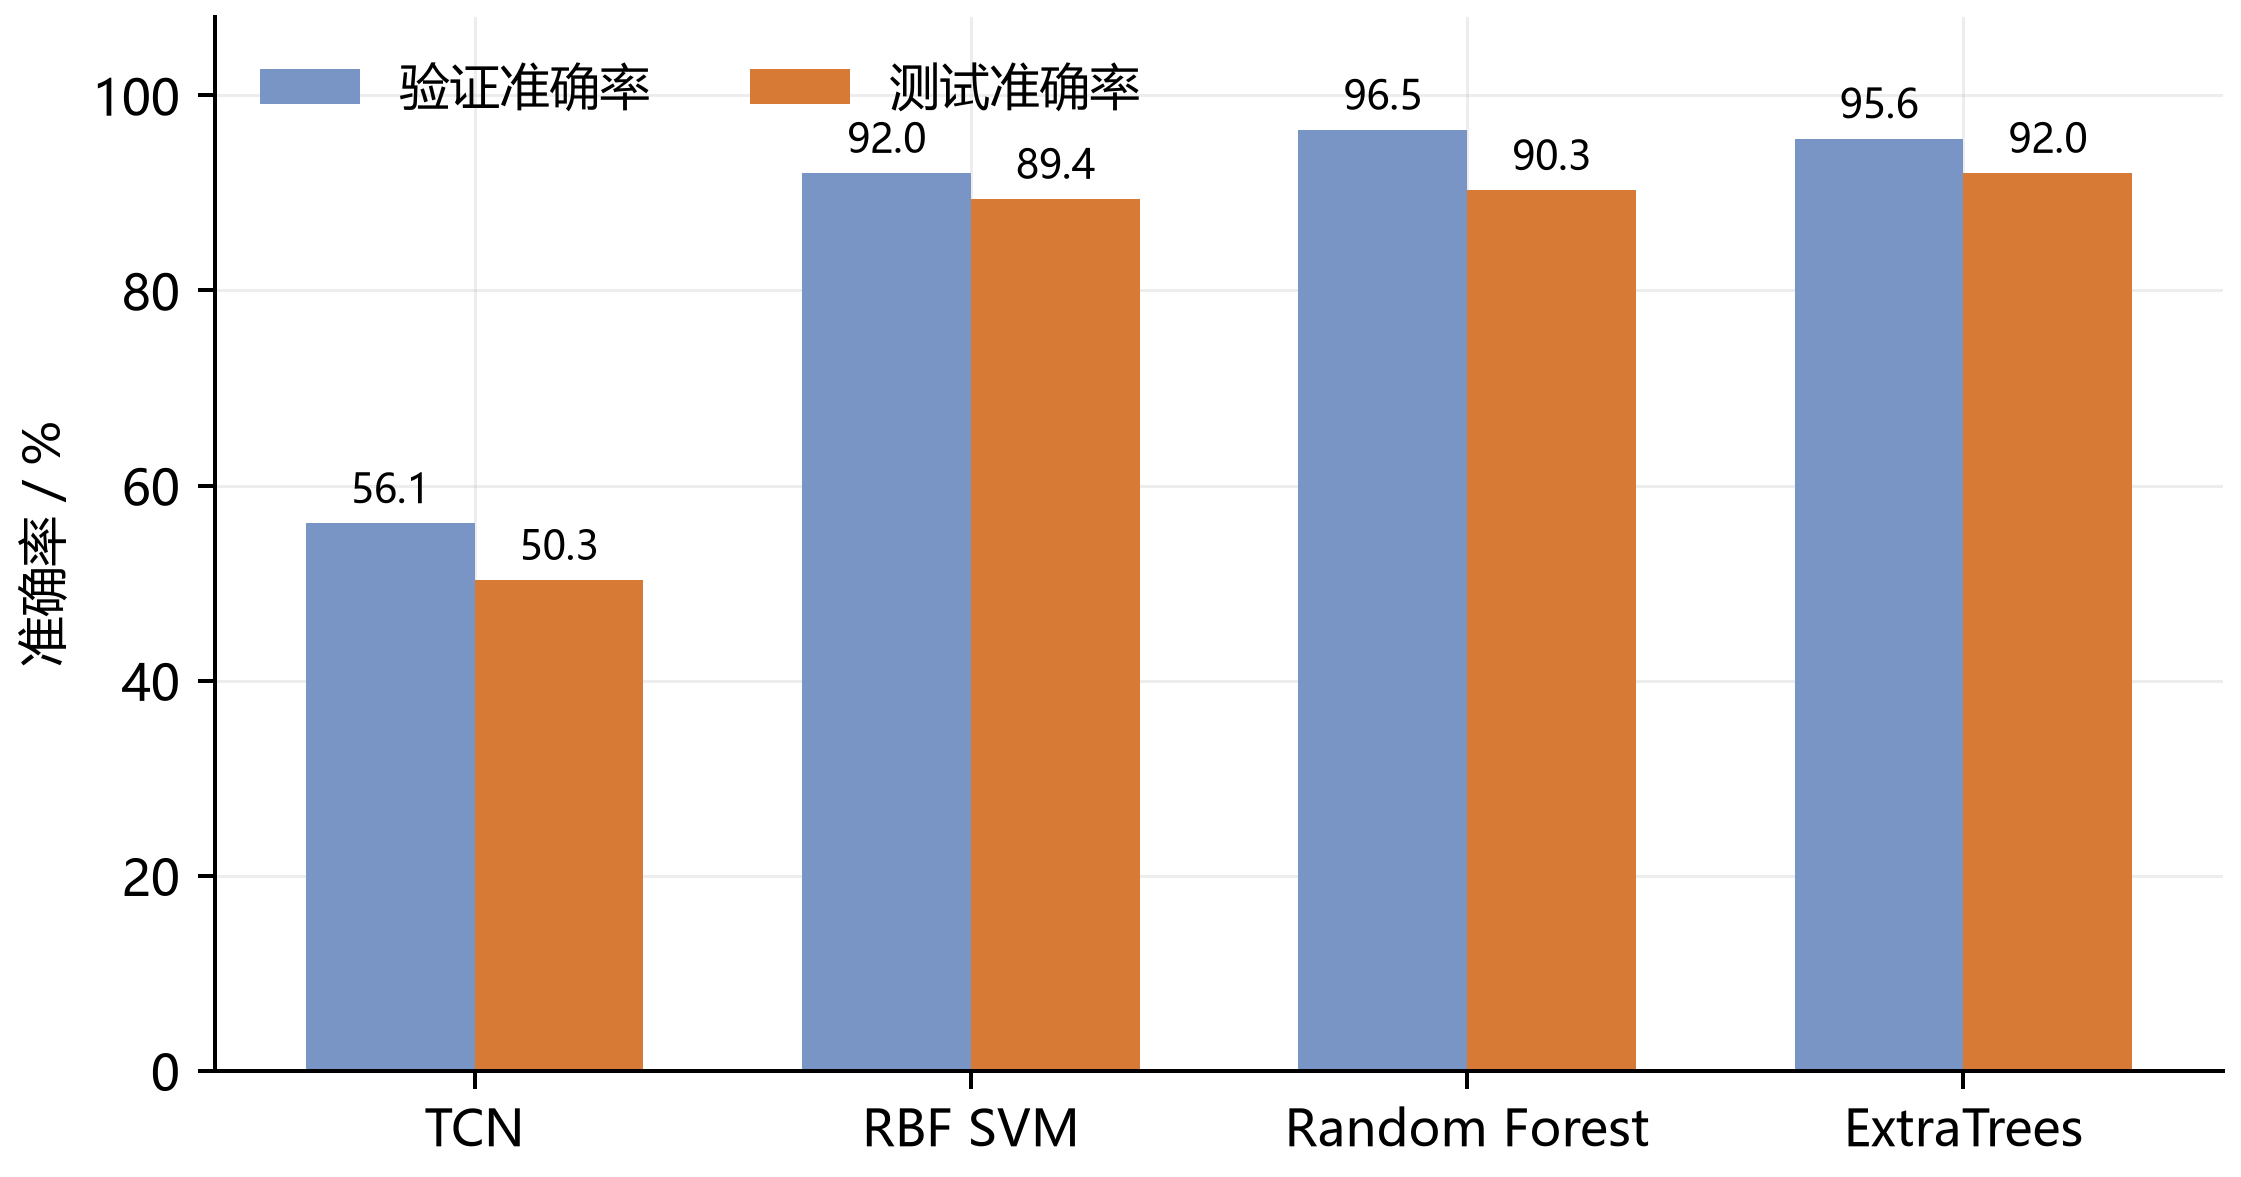
\includegraphics[width=0.88\textwidth]{figures/model_comparison.png}
\caption{不同分类模型的验证集与测试集准确率对比}
\label{fig:model_comparison}
\end{figure}

从实验结果可以看出，TCN 在当前数据规模下测试表现较低，说明仅使用窗口级深度模型难以稳定学习到可泛化的姿态差异。RBF SVM 和 Random Forest 在文件级统计特征上表现明显提升，其中 Random Forest 测试准确率已达到 90.27\%。ExtraTrees 进一步取得 92.04\% 的测试准确率和 92.08\% 的宏平均 F1 值，因此本文选用 ExtraTrees 作为最终分类模型。

\section{最终测试结果}
最终 ExtraTrees 模型在 113 个测试文件上正确分类 104 个文件，测试准确率为 92.04\%。各类别的精确率、召回率和 F1 值如表 4.3 所示。

\begin{table}[htbp]
\centering
\song\wuhao
\caption{ExtraTrees 模型测试集分类结果}
\label{tab:final_result}
\begin{tabular}{ccccc}
\hline
类别 & Precision & Recall & F1 & 正确数/总数 \\
\hline
\texttt{kyphosis} & 87.18\% & 91.89\% & 89.47\% & 34/37 \\
\texttt{normal} & 90.00\% & 94.74\% & 92.31\% & 36/38 \\
\texttt{scoliosis} & 100.00\% & 89.47\% & 94.44\% & 34/38 \\
宏平均 & 92.39\% & 92.03\% & 92.08\% & 104/113 \\
\hline
\end{tabular}
\end{table}

混淆矩阵的类别顺序为 \texttt{kyphosis}、\texttt{normal}、\texttt{scoliosis}，结果为
\begin{equation}
\begin{bmatrix}
34 & 3 & 0 \\
2 & 36 & 0 \\
3 & 1 & 34
\end{bmatrix}.
\end{equation}

\begin{figure}[htbp]
\centering
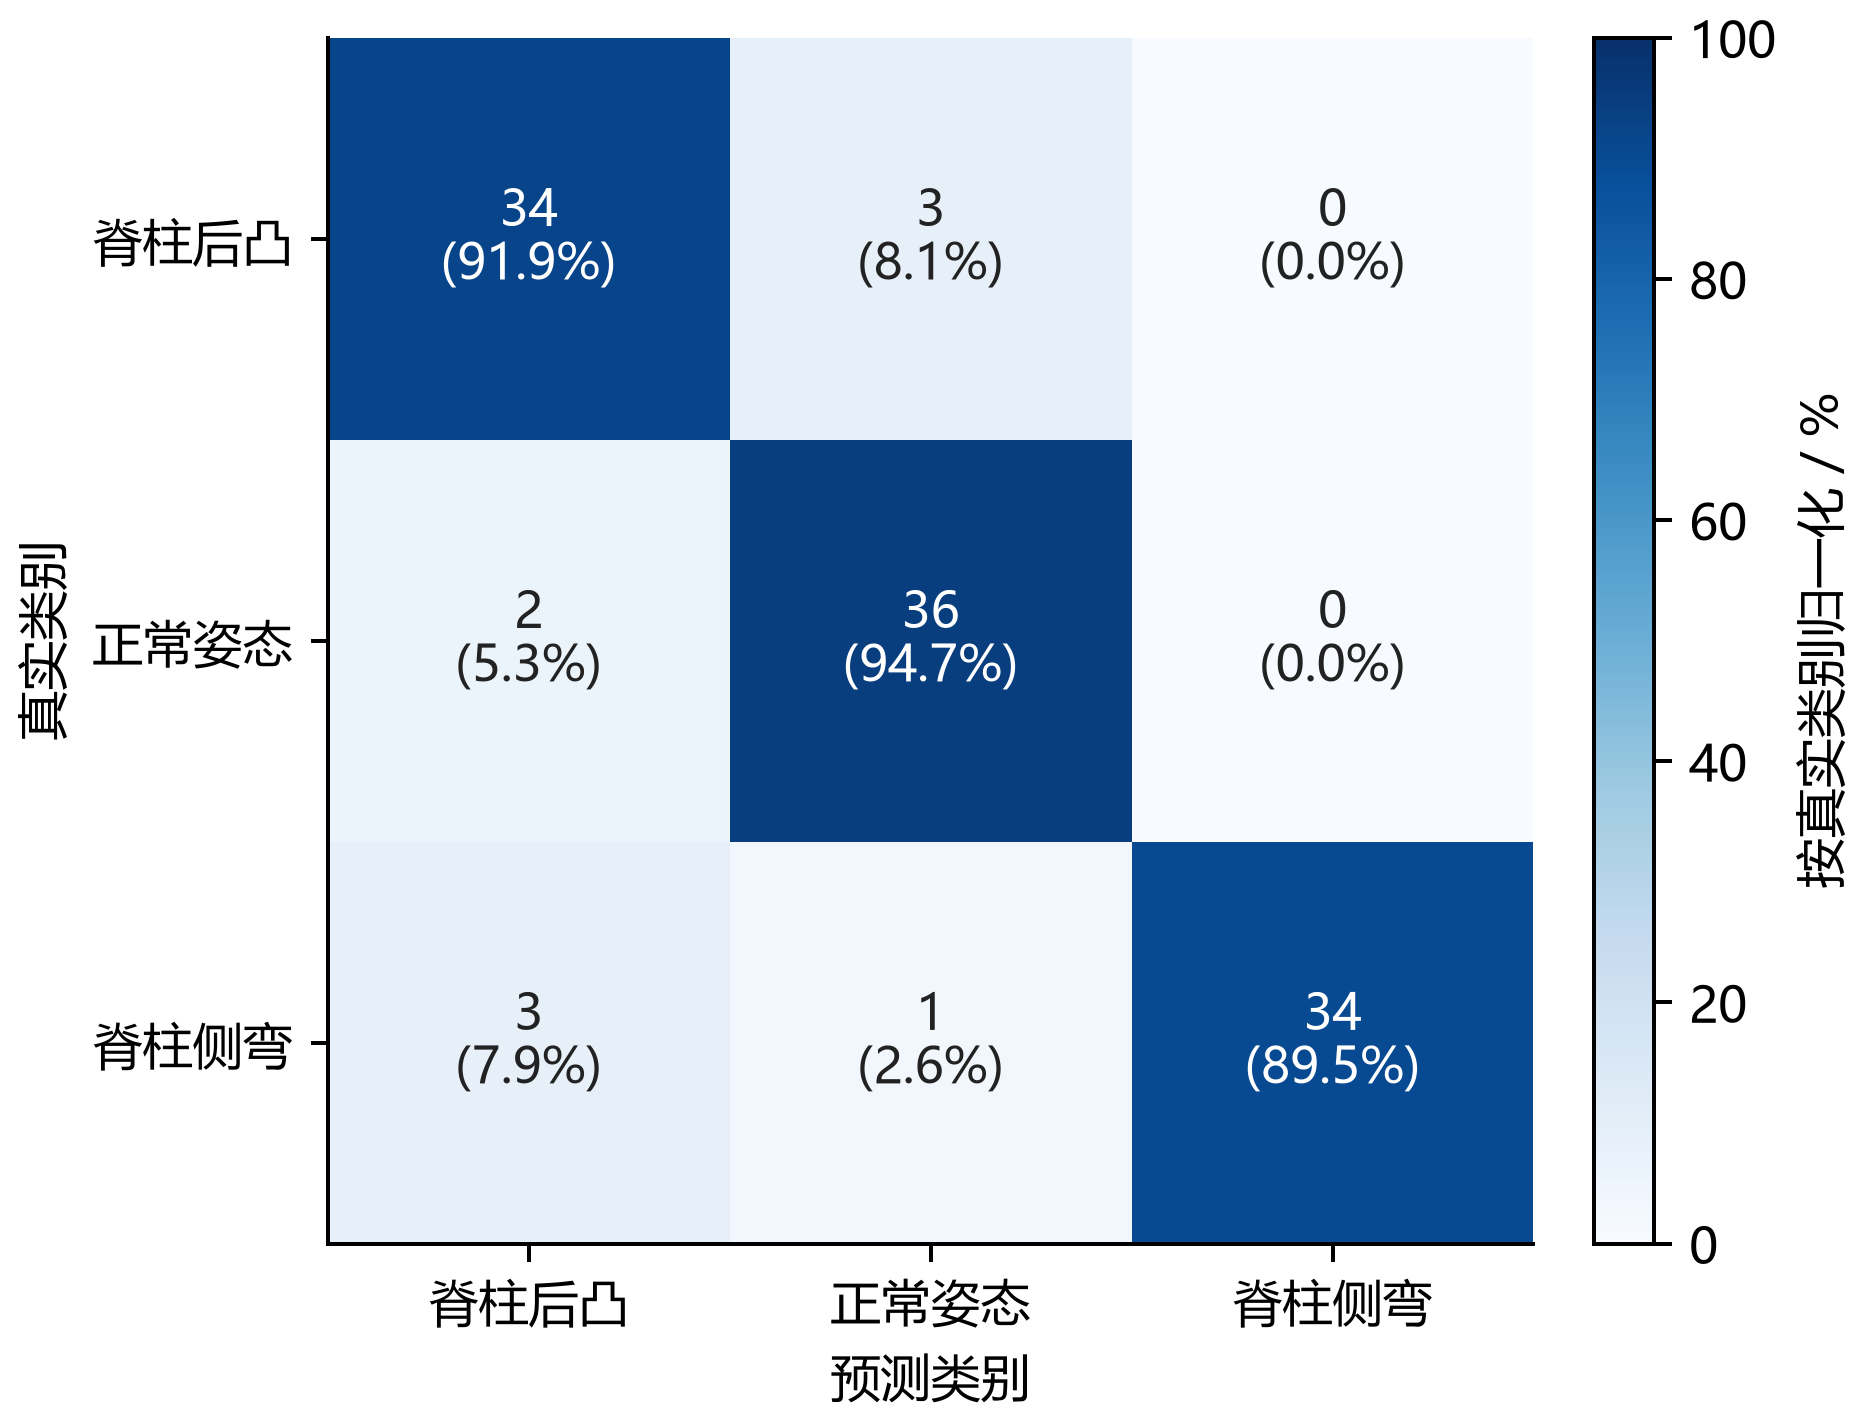
\includegraphics[width=0.72\textwidth]{figures/extratrees_confusion_matrix.png}
\caption{ExtraTrees 模型在测试集上的混淆矩阵}
\label{fig:extratrees_confusion_matrix}
\end{figure}

从混淆矩阵可见，模型对 \texttt{normal} 类别的召回率最高，在 38 个正常姿态测试文件中正确识别 36 个；对 \texttt{scoliosis} 类别的精确率达到 100.00\%，说明测试集中没有其他类别被误判为脊柱侧弯相关姿态；\texttt{kyphosis} 与另外两类之间存在少量混淆，主要表现为 3 个 \texttt{kyphosis} 文件被预测为 \texttt{normal}，以及 3 个 \texttt{scoliosis} 文件被预测为 \texttt{kyphosis}。

\section{结果分析}
实验结果表明，相位比统计特征能够较好地捕捉不同脊柱姿态对 WiFi 信道造成的差异。文件级聚合将多个窗口中的局部时间变化转化为稳定统计量，使模型能够利用完整采集文件中的整体特征进行判断。相比窗口级 TCN，ExtraTrees 在当前数据规模下具有更好的稳定性和测试集表现。

ExtraTrees 的优势主要体现在三个方面。第一，树集成模型适合处理高维统计特征，不需要像神经网络一样从有限样本中重新学习大量时序表示参数。第二，ExtraTrees 的随机特征选择和随机切分阈值能够降低树之间的相关性，提高集成模型的泛化能力。第三，模型训练和推理成本较低，便于在普通 CPU 环境中完成训练、复测和部署。

当前测试结果对应文件级留出测试条件，5 位受试者均出现在训练集、验证集和测试集中。因此，该结果反映的是已登记受试者在相近采集环境下的三类姿态识别能力。后续若面向完全陌生受试者部署，可进一步扩大受试者数量，并采用按受试者分组的划分方式评估跨人泛化能力。

\section{误差模式与结果解释}
从逐类结果看，三类姿态并未表现出完全相同的错误模式。某一类别具有较高精确率，表示模型较少将其他类别误判为该类别；具有较高召回率，则表示该类别的大部分真实样本能够被识别。精确率和召回率所回答的问题不同，因此不能仅根据其中一个指标判断类别识别是否可靠。

混淆矩阵中出现的错误可能来自多种因素。一方面，不同姿态的无线信道分布可能存在重叠，尤其当躯干形态差异较小或受试者保持姿态不稳定时；另一方面，人员体型、相对位置、轻微运动和环境多径也可能改变特征。仅凭混淆矩阵无法确定单个错误的物理原因，若要建立更强解释，需要结合原始信号质量、采集记录和重复实验进行分析。

模型在当前测试集上的结果说明所选特征与分类器在给定条件下具有可行性，但单次文件级随机划分不能估计跨人员性能，也不能充分量化随机划分带来的波动。更完整的评价应包括多次重复划分、置信区间、按受试者分组验证和跨环境测试。由于这些结果尚未在本文当前实验中获得，本文不对其性能作推断，而将其作为后续验证方向。

\section{有效性威胁}
内部有效性主要受到数据划分、参数选择和采集一致性的影响。本文通过文件级划分降低重叠窗口泄漏风险，并隔离测试集；但单次固定划分仍可能受到样本组合偶然性的影响。若采集顺序与姿态标签存在固定对应关系，模型还可能学习时间、设备状态或环境变化等非目标因素。因此，后续实验应随机化采集顺序，并通过重复划分或交叉验证检查结果稳定性。

外部有效性主要涉及受试者、环境和设备覆盖范围。当前评价中不同数据子集包含相同受试者，实验结论主要适用于已覆盖人员和相近采集条件。人员体型、衣着、朝向、收发位置、室内布局和无线设备差异均可能改变信道分布。若目标是面向陌生人员或新环境使用，需要通过分组验证和跨域数据验证模型的泛化能力。

构念有效性关注实验标签与研究概念之间的对应关系。本文分类标签表示预先定义的姿态状态，CSI 模型学习的是这些状态对应的无线信道模式，而不是直接测量脊柱曲率或解剖结构。因此，准确率和 F1 值只能用于评价姿态分类任务，不能转换为医学诊断准确率。实际健康应用仍需要专业人员和标准医学检查建立独立的临床有效性证据。

\section{本章小结}
本章按照研究问题、数据划分、评价指标、模型比较和误差解释组织实验。结果表明，文件级相位比统计特征与 ExtraTrees 的组合在当前留出测试条件下取得了较好的分类性能。与此同时，实验结论受到单次划分、已登记受试者和相近采集环境的限制。通过明确实验协议和有效性威胁，可以将当前结果解释为方法可行性证据，而不是对跨人员或临床性能的直接证明。

